%%%%%%%%%%%%%%%%%%%%%%acronym.tex%%%%%%%%%%%%%%%%%%%%%%%%%%%%%%%%%%%%%%%%%
% sample list of acronyms
%
% Use this file as a template for your own input.
%
%%%%%%%%%%%%%%%%%%%%%%%% Springer %%%%%%%%%%%%%%%%%%%%%%%%%%

\Extrachap{Quick Guide}


Use this Quick Guide as a reference to quickly look up enhanced definitions and pointers for easy reference rather than complex description. A study guide companion, if you will.emplate \emph{glossary.tex} together with the Springer document class SVMono (monograph-type books) or SVMult (edited books) to style your glossary\index{glossary} in the Springer layout.

\section{General Security Concepts}
This Domain covers essential security concepts, security considerations in change management processes, and cybersecurity-related fundamentals.

\subsection{Security Controls}
\runinhead{Security Controls: Measures used to protect systems, assets, and information from threats. They are broadly categorized into four main types: technical, managerial, operational, and physical. Each category addresses security from a different perspective, working together to provide comprehensive protection.}
 
\subsection{Technical Controls}
These are security measures implemented using technology. They include hardware, software, and firmware components designed to protect information systems and networks.

\textbf{Examples:} Firewalls, Intrusion Detection Systems (IDS), antivirus software, encryption, access control systems, and security protocols.

\subsection{Managerial Controls}
These controls focus on the administrative and management aspects of security. They involve policies, procedures, and guidelines that guide security practices within an organization.

\textbf{Examples:} Risk assessments, security awareness training, security policies, change management procedures, and incident response planning.

\subsubsection{Operational Controls}
These are the daily practices and procedures that people use to implement and maintain security. They often involve human interaction with systems and processes.

\textbf{Examples:} Security guard patrols. access control procedures (e.g. badge checks), security awareness training for employees, and incident reporting procedures.

\subsubsection{Physical Controls}
These are tangible measures used to protect physical assets, infrastructure, and personnel from unauthorized access, theft, or damage.

\textbf{Examples:} Locks, fences, security cameras, badge readers, and perimeter security measures such as fences, gates, and bollards.

In essence: \textbf{Technical controls} use technology to protect systems, \textbf{managerial controls} guide the overall strategy, \textbf{operational controls} put those strategies into practice, and \textbf{physical controls} protect the physical environment from threat and harm.

\subsection{Security Control Types}

\textbf{Preventive:} These controls aim to prevent an incident from occurring. Examples include access controls (such as passwords and firewalls), encryption, and security awareness training.

Deterrent: These controls discourage attackers by making the attack less appealing or more difficult to penetrate. Examples include security cameras, motion detectors, warning signs, and policies that increase the perceived risk of being caught.

\textbf{Detective:} These controls identify incidents as they occur or after they have occurred. Examples include Intrusion Detection Systems (IDS), log monitoring, and security audits and assessments.

\textbf{Corrective:} These controls restore the systems to their previous operating states after an incident has occurred. Examples include system backups, disaster recovery plans, and incident response procedures.

\textbf{Compensating:} These controls are used when primary controls are not feasible or insufficient. For example, if a system does not have strong access controls, one might implement more frequent security audits as a compensating control.

\textbf{Directive:} These controls enforce policies and procedures, such as mandatory security training and requiring multifactor authentication.

\runinhead{CIA} Known as the CIA Triad. \textbf{Confidentiality, Integrity, Availability} The CIA triad is a model used in information and cybersecurity to guide policies for protecting data and information. The three core principles work together to ensure that information is protected from unauthorized access, modified only by authorized individuals, and accessible when needed.

\runinhead{AAA} \textbf{Authentication, Authorization, Accounting / Accountability:} AAA is a security framework composed of Authentication, Authorization and Accounting processes. It is a system used to control access to network resources, enforce policies, track usage, and facilitate operational processes. In essence, AAA verifies \textit{who a user is} (authentication, \textit{what they are allowed to do} (authorization), and \textit{how they use} the system (accounting). A breakdown of each component:
\begin{itemize}
    \item \textbf{Authentication:} This process verifies the identity of a user or device that attempts to access a network or an information system. Typically, this involves a username and password, but can also include other authentication methods such as biometrics or security tokens.
    \item \textbf{Authorization:} Once authenticated, authorization determines what the user is allowed to do. Describes the specific resources, services, or commands that a user can access or execute.
    \item \textbf{Accounting:} This process tracks user activity, logging session information such as connection time, bandwidth usage, and resources consumed. This information is used for auditing, assessments and capacity planning.
\end{itemize}

\runinhead{Nonrepudiation} A security concept that ensures the integrity and origin of data, providing proof that a specific action or communication occurred and that the originator cannot deny having sent it or the recipient deny having received it. Essentially, it prevents a party from later denying that they performed an action such as sending a message. Key actions of Nonrepudiation include:
\begin{itemize}
    \item \textbf{Proof of Origin:} Demonstrates who sent a message or initiated an action.
    \item \textbf{Proof of Integrity:} Ensures that the message or data have not been tampered with.
    \item \textbf{Proof of Receipt:} Confirms that the intended message was received by the recipient.
\end{itemize}
How Nonrepudiation is achieved:
\begin{itemize}
    \item \textbf{Digital Signatures:} A cryptographic method that binds a user's identity to a message, acting as a digital fingerprint to prevent denial.
    \item \textbf{Hash Functions:} Used to create a unique digital footprint of data, making any changes easily detectable.
    \item \textbf{Timestamps:} Record when an event occurred, preventing disputes about when something happened (or if it did not).
    \item \textbf{Audit Logs:} Detailed records of system activities, capturing who did what, when, and where, helping with investigations and accountability.
    \item \textbf{Certificate Authority (CA):} Trusted third parties that issue and manage digital certificates and signatures, verifying the identity of users and entities.
    \end{itemize}

\runinhead{Gap Analysis} A gap analysis is a method used to assess the difference between an organization's security posture and its desired, or expected, performance. It helps identify areas where a network security posture may be falling short of its goals and allows the development of strategies to bridge or close those gaps. Essentially, it is a comparison of "where you are" versus "where you want to be." 
Key aspects of a gap analysis include:
\begin{itemize}
    \item \textbf{Identifies the gap:} It pinpoints the discrepancies between the current state and the desired state in various areas, such as performance, resources, processes, or technology.
    \item \textbf{Provides a clear picture:} Helps to understand the current situation by measuring factors such as money and labor and comparing them with the desired target or a baseline.
    \item \textbf{Facilitates improvement:} By understanding the security gaps, organizations can develop action plans to address the shortcomings and move toward their goals.
    \item \textbf{Can be used in various contexts:} Gap analysis can be applied to different areas, including product development, strategy planning, human resources, and more.
\end{itemize}

\runinhead{Zero-Trust} Zero trust is a security framework that operates on the principle of \textit{"never trust, always verify."} It assumes that all users and devices, even those inside the network, are potential threats and require continuous verification and authentication for access.
\textbf{Core Principles:}
\begin{itemize}
    \item \textbf{"Never trust, always verify."} No user, device, or application is trusted by default, even if they are inside the network perimeter.
    \item \textbf{Principle of Least Privilege (PoLP):} Users and devices are granted only the minimum level of access necessary to perform their tasks, limiting potential damage and reducing attack surfaces from breaches.
    \item \textbf{Continuous Verification:} Access is not granted based on one-time authentication. Instead, authentication and authorization are verified continuously and dynamically throughout a session.
\end{itemize}
\textbf{How it Works:}
\begin{itemize}
    \item \textbf{1. Identity Verification:} Every access request is authenticated, and the identity of the user or device is verified before access can be granted.
    \item \textbf{2. Contextual Risk Assessment:} Access is determined based on the context of the request, including user behavior, device posture, and location, using AI and machine learning.
    \item \textbf{3. Policy Enforcement:} Access is granted, denied, or adjusted based on the risk assessment in near-real-time.
    \item \textbf{4. Granular Access Control:} Access is granted based on the Principle of Least Privilege (PoLP) and provides users with the minimum access granted to the resources they need.
    \item \textbf{5. Micro-Segmentation:} Network traffic and applications are segmented into smaller, isolated zones, limiting the scope of a potential breach.
    \item \textbf{Continuous Monitoring (ConMon):} The environment is continuously monitored for anomalies and threats, and security policies are adjusted accordingly.
\end{itemize}

\runinhead{Physical Security} Physical security refers to the measures and practices used to protect people, property, and assets from physical threats such as theft, vandalism, destruction, natural disasters, and unauthorized access. It encompasses a range of strategies and technologies designed to protect physical resources and ensure safety and security. Key aspects of physical security include the following items.
\begin{itemize}
    \item \textbf{Access Control:} Restricting entry to authorized personnel through measures such as locks, keycards, biometric scanners, and security personnel.
    \item \textbf{Perimeter Security:} Establishing physical barriers such as fences, walls, and gates to deter and delay unauthorized access.
    \item \textbf{Surveillance and Monitoring:} Employing CCTV cameras, alarms, and other monitoring systems to detect and respond to potential threats.
    \item \textbf{Physical Barriers:} Using physical structures such as doors, windows, and reinforced walls to protect against intrusion and damage.
    \item \textbf{Security Personnel:} Employing security guards or watchdogs to monitor premises, respond to incidents, and provide a visible deterrent.
    \item \textbf{Environmental Controls:} Implementing measures to mitigate the impact of natural disasters such as floods or fires, such as fire suppression systems and flood barriers.
    \item \textbf{Emergency Preparedness:} Developing and implementing plans to respond to various emergencies, including evacuations and first aid.
\end{itemize}

\runinhead{Deception and Disruption Technology} Deception and disruption technology in cybersecurity involves creating realistic decoys and traps to mislead attackers, allowing organizations to detect and respond to threats early, gather threat intelligence, and disrupt malicious activities. It is a proactive approach that complements traditional security measures by shifting the focus from preventing attacks to detecting and responding to them effectively. A more detailed breakdown is provided below.
\textbf{Deception Technology}
\begin{itemize}
    \item \textbf{Concept:} Involves deploying fake assets using honeypots or honeynets to simulate decoy servers, applications, databases, files, credentials, and more that mimic legitimate ones.
    \item \textbf{Purpose:} To deceive and lure attackers away from critical systems, enticing or luring them to more attractive "targets", making them interact with the decoys instead.
    \item \textbf{Benefit:} Early detection of breaches as attackers interact with decoys, providing information about their tactics, techniques and procedures (TTP).
\end{itemize}
Examples include:
\begin{itemize}
    \item \textbf{Honeypots:} Systems designed to attract and trap attackers.
    \item \textbf{Deceptive files:} Files that appear legitimate but, in fact, contain misleading information or trigger alerts upon access.
    \item \textbf{Deceptive email accounts:} Mimicking real email addresses to identify phishing attempts.
    \item \textbf{Deceptive network infrastructure:} Creating fake networks and servers that attract attackers to infiltrate shifting their focus from legitimate network assets to decoys.
\end{itemize}

\runinhead{Change Management} Change management in security refers to a structured process that organizations use to manage and control modifications to their information systems, policies, and procedures to ensure that they do not negatively affect security processes or procedures. It is a way to handle changes in a controlled and coordinated manner, and minimizes risks associated with unauthorized or poorly planned modifications.
Key aspects of change management in security consist of the following processes defined below.
\begin{itemize}
    \item \textbf{Structured Processes:} It involves a defined process for requesting, evaluating, approving, testing, and documenting changes.
    \item \textbf{Risk Mitigation:} Change management aims to reduce the risk of security breaches, system outages, and other negative consequences that can arise from poorly managed changes.
    \item \textbf{Policy and Procedure Updates:} Changes to security policies and procedures are also managed through this process to ensure they align with organizational needs and security best practices.
    \item \textbf{Business Impact Assessment (BIA):} Organizations assess the potential impacts of proposed changes on their security posture before implementing them.
    \item \textbf{Audible Process:} All changes are tracked and documented, allowing for auditing and accountability.
    \item \textbf{Alignment with Business Needs:} Change management ensures that security changes align with the organizations overall business goals and objectives.
    \item \textbf{Tools and Automation:} Many organizations use automated tools and workflows to streamline the change management process.
\end{itemize}
In essence, change management in security is about ensuring that modifications to an organization's security infrastructure and practices are implemented safely and effectively, minimizing risks while supporting business operations.

\runinhead{Ownership} Parties responsible for organizational changes.

\runinhead{Stakeholders} In a cybersecurity context, stakeholders are individuals or groups who have a vested interest in an organization's cybersecurity practices and are affected by its operations. These stakeholders can be internal, such as employees and management, or external, such as customers, suppliers, and regulatory bodies.

\runinhead{Impact Analysis} Impact analysis in cybersecurity refers to the processes of evaluating the potential consequences of a cybersecurity incident or breach on an organization's operations, finances, reputation, and legal standing. It helps organizations to better understand the potential damage from a cyberattack and prioritize resources for mitigation and recovery procedures.

\runinhead{Backout Plan} A backout plan in cybersecurity is a documented procedure that outlines how to revert to a previous system-state, after making changes or updates, ensuring minimal disruption and data integrity. It is a crucial part of cybersecurity as it provides a safety net to mitigate the risks associated with new deployments and modifications to existing infrastructure.

\runinhead{Maintenance Window} A maintenance window is a pre-scheduled recurring or one time period of time when planned maintenance tasks, such as software updates, security patches, and testing system upgrades, are performed on managed or in-production systems. This practice helps minimize disruptions to users and operations by ensuring maintenance is accomplished during defined, less critical operating times.

\runinhead{Standard Operating Procedure (SOP)}  In cybersecurity, a Standard Operating Procedure (SOP) is a documented, step-by-step guide that outlines the specific actions required to maintain and protect an organization's digital assets and infrastructure. SOPs ensure consistency, efficiency, and compliance in handling security incidents, managing digital assets, and adhering to relevant regulations. They essentially provide a standardized approach to security operations, minimizing the risk of human error and ensuring consistent responses to security threats. Key aspects of a cybersecurity SOP may include, but are not limited to:
\begin{itemize}
    \item \textbf{Incident Response:} SOPs detail the steps for detecting, containing, investigating, and resolving security incidents.
    \item \textbf{Threat Intelligence Analysis:} They define how to analyze and respond to emerging cyber threats.
    \item \textbf{Vulnerability Management:} These SOPs outline the process for identifying, assessing, and mitigating vulnerabilities.
    \item \textbf{Access Control:} They cover procedures for managing user and device access, authentication, and authorization.
    \item \textbf{Security Monitoring:} SOPs specify how to monitor systems and networks for suspicious activities.
    \item \textbf{Data Protection:} They include guidelines for handling sensitive information and protecting digital assets.
    \item \textbf{Compliance:} SOPs help organizations adhere to relevant security regulations and standards.
\end{itemize}

%\runinhead{Allowlists and Denylists} In cybersecurity, allow lists (formerly known as \textit{"whitelists")} and denylists (formerly known as \textit{"blacklists")} are used to control access to resources and systems. Allowlists define what is permitted, while denylists define what is blocked.
\textbf{Allowlists}
\begin{itemize}
    \item \textbf{Definition:} An allowlist specifies the entities (users, applications, IP addresses, and more) that are explicitly permitted to access a resource or perform a specific action.
    \item \textbf{Approach:} It operates on a "deny by default, allow by exception" principle. Everything is first blocked unless it is explicitly listed as allowed.
    \item \textbf{Security:} Offers a higher level of security because only known and trusted entities are granted access.
    \item \textbf{Maintenance:} Requires more effort to maintain, as every new entity must be added to the list to be allowed.
    \item \textbf{Use Cases:} Suitable for scenarios where strict access control is required, such as controlling access to sensitive data or critical systems.
\end{itemize}
\textbf{Denylists}
\begin{itemize}
    \item \textbf{Definition:} A denylist specifies the entities that are blocked or restricted from accessing a resource or performing a specific action.
    \item \textbf{Approach:} Operates on a "allow by default, deny by exception" principle. Everything is permitted unless it is explicitly listed as blocked.
    \item \textbf{Security:} Easier to implement and maintain but offers a lower level of security, as it relies on identifying and blocking only known threats.
    \item \textbf{Maintenance:} Easier to maintain as you only need to add malicious entities to the list to block them.
    \item \textbf{Use Cases:} Suitable for scenarios where you need to block known threats such as malware or spam, but do not require strict control over all access.
\end{itemize}
In essence:
\begin{itemize}
    \item Allowlists are more secure but require more management.
    \item Denylists are easier to manage but offer less security.
\end{itemize}
Both allowlists and denylists are valuable tools in cybersecurity, and the choice of which to use depends on the specific security requirements of the system or application.

\runinhead{Public Key Infrastructure (PKI)} PKI, or Public Key Infrastructure, is a system that enables secure online communications and transactions using digital certificates and cryptography. PKI establishes trust and verifies the identity of individuals, devices, and services, by using a pair of cryptographic keys: a public key for encryption and a private key for decryption. PKI is essential to secure websites, email, documents, and other digital assets. Key concepts include:
\begin{itemize}
\item \textbf{Asymmetric Cryptography:} PKI relies on asymmetric cryptography which uses two mathematically related keys: \textbf{public key} and a \textbf{private key.}
\item \textbf{Digital Certificates:} These are electronic documents that bind a public key to a specific entity, such as a person, device, or organization. Certificates are issued by a trusted third-party called a \textit{Certificate Authority (CA).}
\item \textbf{Private Key:} This key is kep secret and hidden by the entity and is used to decrypt messages that are encrypted with their corresponding public key or to digitally sign documents.
\item \textbf{Public Key:} This key is freely available and can be used by anyone to encrypt messages or verify digital signatures created with the corresponding private key.
\end{itemize}

\runinhead{Encryption Levels} Encryption levels for full disk, partition, file, volume, and database all depend on the specific implementations and generally involve algorithms such as AES (Advanced Encryption Standard) (with varying key lengths such as 128-bit, 192-bit, or 256-bit) or other encryption methods. Full Disk Encryption (FDE) often uses XTS-AES, while volume encryption might use AES-128, AES-192, or AES-256. Database encryption can involve \textit{ Transparent Data Encryption (TDE)} or \textit{Column-Level Encryption (CLE).}
\textbf{Full Disk Encryption (FDE):}
\begin{itemize}
    \item \textbf{Encryption Algorithms:} Commonly uses AES-256-XTS, AES-128, or AES-CBC (Cipher Chain Block).
    \item \textbf{Key Lengths:} 128-bit or 256-bit AES keys.
    \item \textbf{Focus:} Protects all data on the entire hard drive.
    \item \textbf{Implementation Examples:} Hardware-based FDE (e.g., using OPAL and Enterprise standards), software-based FDE (e.g., BitLocker, VeraCrypt).
\end{itemize}
\textbf{Partition Encryption:}
\begin{itemize}
    \item \textbf{Encryption Algorithms:} Similar to FDE and use AES, XTS-AES.
    \item \textbf{Key Lengths:} Similar to FDE, encryption can vary.
    \item \textbf{Focus:} Protects data within a specific partition of a hard drive.
    \item \textbf{Implementation Examples:} BitLocker, FileVault, TrueCrypt, PGP.
\end{itemize}
\textbf{File Encryption:}
\begin{itemize}
    \item \textbf{Encryption Algorithms:} Depends on the implementation, can include AES and other algorithms.
    \item \textbf{Key Lengths:} Depends on the algorithm and implementation.
    \item \textbf{Focus:} Protects individual files or groups of files.
    \item \textbf{Implementation Examples:} EFS (Windows), fscrypt (Linux), file encryption within cloud-based storage.
\end{itemize}
\textbf{Database Encryption:}
\begin{itemize}
    \item \textbf{Encryption Algorithms:} Transparent Data Encryption (TDE), Column-Level Encryption (CLE), AlwaysEncrypted (SQL Server).
    \item \textbf{Key Lengths:} Depends on the chosen encryption method and algorithm.
    \item \textbf{Focus:} Encrypts data within a database management system (DBMS).
    \item \textbf{Implementation Examples:} Transparent Data Encryption (TDE) in SQL Server, Column-Level Encryption (CLE).
\end{itemize}

\runinhead{Symmetric Ciphers} Symmetric ciphers, also known as \textbf{symmetric-key algorithms}, use the same secret key for encryption and decryption. This makes them efficient and fast for encrypting large volumes of data.
\textbf{Types of Symmetric Ciphers}
Symmetric ciphers are generally categorized as either \textbf{stream ciphers} or \textbf{block ciphers}.
\textbf{Stream Ciphers}
\begin{itemize}
    \item \textbf{RC4:} RC4 (Rivest Cipher 4) is a stream cipher that generates a pseudorandom keystream and XORs it with the plaintext and creates ciphertext. It is known for its simplicity and speed, making it suitable for applications where rapid encryption and decryption are essential.
    \item \textbf{How it Works:} Stream ciphers encrypt data one bit or byte at a time. RC4 utilizes a Key Scheduling Algorithm (KSA) to initialize a state array, which is then used by a Pseudo-Random Generation Algorithm (PRGA) to produce the keystream. This keystream is then XORed with the plaintext to generate the ciphertext.
    \item \textbf{Considerations:} While once widely used, RC4 has been found to have significant vulnerabilities and is no longer recommended for strong security applications.
\end{itemize}
\textbf{Block Ciphers}
Block ciphers operate on fixed-size blocks of data, encrypting each block independently using the same key.
\begin{itemize}
    \item \textbf{DES:} The Data Encryption Standard (DES) is a block cipher that encrypts data in 64-bit blocks using a 56-bit key.
        \item \textbf{How it Works:} DES utilizes a 16-round Feistel network for encryption and decryption, involving a series of substitutions and permutation operations.
        \item \textbf{Considerations:} DES is considered outdated and vulnerable due to its short key length, making it easily crackable and susceptible to brute-force or Man-in-the-Middle (MiTM) attacks.
    \item \textbf{Blowfish:} Blowfish is a symmetric block cipher designed by Bruce Schneier. It uses a 64-bit block size and a variable-length key ranging from 32 to 448 bits.
        \item \textbf{How it Works:} Blowfish employs a 16-round Feistel cipher structure with key-dependent S-boxes and a complex key schedule.
        \item \textbf{Considerations:} Blowfish is considered secure for smaller files, but its 64-bit block size could be vulnerable to Sweet32 birthday attacks, particularly when encrypting files larger than 4GB.
    \item \textbf{3DES:} Triple DES (3DES), or Triple Data Encryption Algorithm (TDEA), applies the DES algorithm three times to each data block. This significantly increases the effective key length and security compared to DES.
        \item \textbf{How it Works:} 3DES uses three different keys, applying DES encryption with the first, DES decryption with the second, and DES encryption again with the third (for the strongest variant).
        \item \textbf{Considerations:} Although considered more secure than DES, 3DES is slower and more computationally intensive. It also remains susceptible to certain attacks, such as Sweet32. NIST has since deprecated 3DES and disallowed its use (except for processing already encrypted data) by the end of 2023.
\end{itemize}
\textbf{General Considerations for Symmetric Ciphers}
\begin{itemize}
    \item \textbf{Key Length:} The strength of a symmetric cipher is directly related to its key length. Longer keys offer greater resistance to brute-force attacks.
    \item \textbf{Block Size:} For block ciphers, the block size determines how much data is processed at each step.
    \item \textbf{Number of Rounds:} Many block ciphers, including DES and AES, employ multiple rounds of encryption operations. Increasing the number of rounds typically enhances the security strength of the cipher.
\end{itemize}
\textbf{ Modern Alternatives}
The Advanced Encryption Standard (AES) has replaced DES and 3DES as the standard symmetric encryption algorithm. It is also used by the United States Federal Government as their preferred encryption method (AES-256). AES offers vastly larger key sizes (128, 192, and 256 bits) and a more complex, efficient design. AES is generally recommended for modern applications because of its robust security and efficiency. Newer stream ciphers, such as Salsa20 and ChaCha20, are also considered far more secure alternatives to RC4.

\runinhead{Asymmetric Ciphers} Asymmetric ciphers, also known as \textit{Public-Key Cryptography)}, use pairs of mathematically related keys: a \textbf{public key that can be shared openly} and a \textbf{private key that must be kept private and secret}; examples of asymmetric ciphers include RSA, Diffie-Hellman key exchange, and Elliptic Curve Cryptography (ECC) where anyone can use the public key to encrypt a message, but only the holder of the corresponding private key can decrypt it. Points on asymmetric ciphers:
\begin{itemize}
    \item \textbf{RSA:} RSA, or Rivest-Shamir-Adelman cipher is one of the most widely used asymmetric ciphers, based on the difficulty of factoring large prime numbers.
    \item \textbf{Diffie-Hellman (DH):} Primarily used for key exchange, allowing two parties to securely establish a shared secret key over a public channel.
    \item \textbf{Elliptic Curve Cryptography (ECC):} Offers similar security to RSA but with smaller key sizes, making it more efficient for applications with limited bandwidth.
\end{itemize}

\runinhead{Trusted Platform Module (TPM)} A Trusted Platform Module (TPM) is a specialized chip on a computer's motherboard designed to enhance security by storing cryptographic keys used for encryption and decryption. It acts as a secure vault for sensitive information, such as encryption keys, passwords, and certificates. TPMs are tamper resistant and help ensure the integrity of the platform, particularly during the boot process.
\textbf{Core Functions}
\begin{itemize}
    \item \textbf{Secure Key Storage:} TPMs store cryptographic keys (such as those used for encryption) securely, preventing them from being accessed by unauthorized software or users.
    \item \textbf{Platform Integrity:} TPMs can verify the integrity of the system's hardware and software, ensuring that the boot process starts from a trusted state and hasn't been tampered with.
    \item \textbf{Cryptographic Operations:} TPMs can perform cryptographic operations such as  encryption, decryption, and hashing, which are essential for security functions.
    \item \textbf{Random Number Generator:} TPMs can also generate random numbers, which are used in various security protocols.
\end{itemize}
\textbf{How it Works}
\begin{itemize}
    \item \textbf{Hardware-Based Security:} TPMs are hardware components that make them more resistant to software-based attacks than purely software-based security solutions.
    \item \textbf{Integration with OS and Applications:} TPMs work in conjunction with the operating system and applications to provide security features.
    \item \textbf{Trusted Boot:} One of the main uses of TPMs is in secure boot, where the TPM verifies the integrity of the boot process and ensures that the operating system hasn't been tampered with or modified in any way.
    \item \textbf{Encryption:} TPMs can be used to encrypt hard drives, protect files and folders, and enhance other security features such as a VPN (Virtual Private Network and remote access.
\end{itemize}
In essence, a TPM is a hardware security module that acts as a trusted anchor for a computer system, enhancing its security and protecting sensitive information.

\runinhead{Secure Enclave} A secure enclave in computer networks refers to an isolated hardware-based environment within a computing system designed to protect sensitive data and code. It acts as a \textit{ Trusted Execution Environment (TEE)} with minimal attack surface, where critical operations are carried out in a secure and isolated manner. This isolation helps prevent unauthorized access, modification, or disclosure of sensitive information, even if the main operating system or other parts of the system are compromised.

\runinhead{Steganography} Steganography is the practice of concealing a message within another message or physical object, making the hidden message imperceptible to an observer without special knowledge. It is essentially "covered writing," using the term from Greek roots, and can involve hiding data in various formats such as images, audio, or even text. It is basically a hidden text or meaning obscured under a primary means such as an image or audio file, and is normally not something the human eye can immediately see.
\textbf{Core Concept:} Steganography aims to hide the very existence of a message, as cryptography does and focuses on making a message unreadable in human format without a key. Examples include:
\begin{itemize}
    \item \textbf{Digital Steganography:} Hiding a secret message within an image file by altering the least significant bits of the color data, or embedding data within the metadata file.
    \item \textbf{Physical Steganography:} Using invisible ink, microdots, or writing behind stamps to conceal alternative, second hidden, embedded message.
\end{itemize}
\textbf{How it Works}
\begin{itemize}
    \item \textbf{Cover Object:} The original file or object that will contain the hidden message.
    \item \textbf{Secret Message:} The data that need to be hidden.
    \item \textbf{Steganographic Algorithm:} The method used to embed the secret message within the cover object.
\end{itemize}
\textbf{Common Techniques}
\begin{itemize}
    \item \textbf{LSB Replacement:} Replacing the least significant bits of the cover object with the bits of the secret message.
    \item \textbf{Word/Letter Substitution:} Hiding a message by strategically placing words or letters within a larger text.
\end{itemize}
\textbf{Key Differences in Cryptography}
\begin{itemize}
    \item \textbf{Concealment of existence versus readability:} Steganography aims to hide the fact that a message exists, while cryptography focuses on making the message "unlockable" or unreadable.
    \item \textbf{Techniques:} Steganography uses techniques to embed data within a cover object, while cryptography uses encryption algorithms.
    \item \textbf{Application:} Steganography is often used for covert communications, while cryptography is used to protect the confidentiality and integrity of original messages.
\end{itemize}

\runinhead{Tokenization} Tokenization is a data security process that replaces sensitive unique identifiers with sensitive information called \textbf{tokens}. These tokens have no exploitable value and can be safely stored, reducing the risk of data compromise. It is a form of data protection that replaces sensitive data with a random placeholder, which can then be used in place of the original data. A more detailed explanation is offered below.
\textbf{In Data Security:}
\begin{itemize}
    \item \textbf{Replacing Sensitive Data:} Tokenization replaces sensitive data such as credit card numbers, social security numbers, or personally identifiable information with random nonsensitive tokens.
    \item \textbf{No Reversible Process:} Unlike encryption, tokenization is not mathematically reversible; therefore, it technically cannot be reverse-engineered. It does not use a key to decrypt the data back to its original form.
    \item \textbf{Security and Convenience:} Tokenization enhances security by keeping the original sensitive data in a secure vault while using tokens to process transactions or store data.
    \item \textbf{Examples:} Tokenization is widely used in payment processing, where credit card numbers are replaced with tokens during transactions. It is also used for mobile and digital cryptocurrency wallets, and in e-commerce.
    \item \textbf{Benefits:} Tokenization reduces the risk of data or PII (Personally Identifiable Information) breaches, simplifies compliance with data security and privacy regulations, and improves transactional processing speeds and conveniences.
\end{itemize}

\runinhead{Data Masking} Data masking is the process of obscuring sensitive data to protect while still allowing use for other purposes, such as testing or analysis. Sensitive information is replaced with realistic but fictitious data, preventing unauthorized access while maintaining the usability of the data. A more detailed explanation is offered below.
\begin{itemize}
    \item \textbf{What it Protects:} Data masking protects sensitive information such as real names, addresses, social security numbers, credit card numbers, and other confidential data.
\end{itemize}
\textbf{How it Works}
\begin{itemize}
    \item \textbf{Replacing sensitive data:} Instead of storing or using real sensitive data, data masking techniques replace it with fictional or altered data.
    \item \textbf{Maintaining usability:} While the data is masked, it still retains some characteristics of the original data, allowing realistic testing and analysis.
    \item \textbf{Types of Masking:}
    Data masking can be achieved through the various methods, including:
        \item \textbf{Substitution:} Replacing real data with similar, but fictitious data.
        \item \textbf{Shuffling:} Randomizing the order of characters within a field of characters.
        \item \textbf{Redaction:} Completely overwriting sensitive data with placeholder characters.
        \item \textbf{Encryption:} Replacing data with ciphertext that requires a key for decryption.
        \item \textbf{Hashing:} Generating a fixed size value from the original data, making it irreversible.
\end{itemize}
\textbf{Use Cases}
Examples include:
\begin{itemize}
    \item Replace a customer's real name with a randomly generated name from a predefined list.
    \item Mask social security numbers with asterisks (e.g. 123-45-****), while still retaining the last four digits for identification.
    \item Using encryption to protect sensitive data while at rest or in transit.
    \item Replace employee salaries with the average salary for their role.
\end{itemize}

\runinhead{Hashing} Hashing is a process that converts data of any size into a fixed-size string of characters using a mathematical function, often called a \textbf{ hash function}. This process is generally irreversible because it is extremely difficult to retrieve the original data from the resulting hash. Hashing is widely used in cyber security and ethical hacking for password storage, data integrity checks, and digital signatures. A more detailed explanation is offered below.
\begin{itemize}
    \item \textbf{Hash Function:} This is the algorithm that takes the input data and transforms the data into a unique fixed-size string called a \textit{hash} or \textit{hash value}.
    \item \textbf{One-Way Function:} A key characteristic of hashing is that it is a one-way function. This is because it is computationally infeasible to reverse the process and obtain the original data from the hash.
    \item \textbf{Data Integrity:} Hashing is used to verify data integrity. If the hash of a file or message changes, it indicates modification of data.
    \item \textbf{Password Storage:} Instead of storing passwords in plaintext (which is highly vulnerable), systems store the hash of the password. When a user enters their password, it is hashed and compared to the stored hash, ensuring secured authentication.
    \item \textbf{Digital Signatures:} Hashing is used to create digital signatures. The hash of a document is encrypted with the sender's private key, creating a signature that verifies the document's origin and ensures it has not been tampered with.
\end{itemize}
Some examples include:
\begin{itemize}
    \item Common hashing algorithms include MD5, SHA-256, and bcrypt.
\end{itemize}

\runinhead{Salting (Salts)} Salting is a security measure used when storing passwords. It involves adding a random, unique string of characters (the "salt") to a user's password before it is hashed and stored. This makes it much harder for attackers to crack passwords, even if they gain access to the hashed password database, by preventing the use of pre-computed hash tables (such as rainbow tables) and making it necessary to compute each hash individually, which proves to computationally infeasible many times. A more detailed explanation is offered below.
\begin{itemize}
    \item \textbf{Salting is a cryptographic technique:} It is a method to add extra randomness to the password storage process and is considered a defense-in-depth or a layered security approach.
    \item \textbf{Hashing:} The salt is combined with the password and this combined string is then passed through a hashing algorithm (such as SHA-256).
    \item \textbf{Example:} If two users have the password "password" but different salts applied, their hashed passwords will be completely different.
    \item \textbf{Storing the salt:} The salt is stored with the hashed password, allowing the system to retrieve the salt when verifying a user's logon attempt.
    \item \textbf{Login process:} When a user logs in, the system retrieves the salt associated with their username, combines it with the password they entered, hashes the combined string, and compares it to the stored hash.
\end{itemize}

\runinhead{Digital Signature (DS)} A digital signature is a mathematical scheme that verifies the authenticity and integrity of digital messages or documents. It is essentially a secure way to prove that a document came from a specific sender and has not been tampered with. Digital signatures are used in various applications, such as emails, sensitive PDFs, financial transactions, and software distribution. A detailed explanation is offered below.

\section{How it Works}

\subsection{Public-Key Cryptography}
\begin{itemize}
    \item Digital signatures rely on public-key cryptography, also known as \textbf{asymmetric cryptography}, that use a pair of keys: a \textbf{ private key for signing} and a \textbf{public key for verification}. 
\end{itemize}

\subsection{Hashing}
\begin{itemize}
    \item Before signing, the document is first "hashed," creating a unique digital fingerprint (a fixed-length string).
\end{itemize}

\subsection{Signing} 
The sender uses their private key to encrypt the hash of the document, creating the digital signature.

\subsection{Verification}
The recipient uses the sender's public key to decrypt the signature and compare it to a new hash calculated from the received document. If the hashes match, it confirms the document's authenticity and integrity.

Often, digital signatures are linked to digital certificates, which contain the sender's public key and identity information. These certificates, issued by trusted third parties (Certificate Authorities (CAs), further enhance the trustworthiness of the signature.

\textbf{Note:} \textit{Digital signatures are legally binding. In many jurisdictions, digital signatures are legally recognized as equivalent to handwritten signatures.}

\runinhead{Key Stretching} Key stretching is a cryptographic technique used to strengthen weak keys, usually passwords, by making them more resistant to brute-force and dictionary attacks. It involves repeatedly applying a cryptographic function to the key, effectively increasing its length and complexity, making it more computationally expensive to crack. A detailed explanation is offered below.
\begin{itemize}
    \item \textbf{Weak Keys:} Passwords, especially short or simple ones, are considered weak keys because they can be easily guessed or cracked by attackers.
    \item \textbf{Key Stretching Process:} Key stretching algorithms, such as \textbf{PBKDF2} or \textbf{Argon2}, take a weak key (for example, a password) and apply a hashing function multiple times. This process is repeated hundreds or thousands of times.
    \item \textbf{Increased Computational Effort Required:} The repeated hashing significantly increases the time and computational resources needed to crack the key. Even if an attacker has access to the stretched key, they would need considerably more time and processing power to try and reverse engineer the process. This feat, in turn, also means that the attacker needs to be a specialist in reverse engineering software, programs, and cryptography, which is very complex to master.
\end{itemize}

\section{Examples of Key Stretching Algorithms:}
\begin{itemize}
    \item \textbf{PBKDF2:} Password-Based Key Derivation Function 2, a widely used key stretching algorithm, which combines hashing with salting.
    \item \textbf{Argon2:} A more recent and secure algorithm, known for its memory-hardness, which means that it requires significant memory to compute.
\end{itemize}
\textbf{Salting:} Key stretching often incorporates salting, which involves adding a random value (salt) to the key before hashing. This adds another layer of complexity and makes it harder for attackers to use precomputed hash tables of common passwords.

\runinhead{Pepper} A pepper is a secret fixed value (like a long, random string) added to a password before it is hashed. Unlike a salt, which is stored with the password hash, a pepper is kept separate and often hardcoded in the application or stored securely elsewhere. This adds additional layers of security, making it more difficult to crack even if access to the password database has occurred. A detailed explanation is offered below.

\section{Salting Versus Peppering}
Both salting and peppering are techniques used to enhance password security by making it more difficult to crack passwords using precomputed hash tables. Salting adds a random string to the password \textit{before} hashing, and this salt is stored alongside the hashed password in the database. Peppering, on the other hand, involves adding a secret, fixed value (the pepper) to the password, but this pepper is not stored with the password hash.

\section{How it Works}
When a user enters a password, the system combines it with the pepper (using the same method used during account creation) and then hashes it. The resulting hash is compared to the stored hash.

\textbf{Security Benefits:} If an attacker gains access to the database, they will have the salts and hashed passwords, but they will still need the pepper to crack the passwords. If the pepper is securely stored and is not easily accessible, it can significantly increase the difficulty and processing power needed to crack the password.

%\textbf{Example:} Imagine that a website uses a pepper such as \texttt{"5965937f-47d8-4f9b-92e4-802972f47650."} When a user with the password "\texttt{password123"} logs in, the system might combine it with the pepper (e.g. \texttt{"password1235965937f-47d8-4f9b-92e4-802972f47650"}) and then hash it. The resulting hash is then compared with the stored hash.

Implementation: While peppering offers good security, it is not commonly implemented along with salting. Some hashing libraries might not directly support it. The main downside is that the pepper needs to be managed securely and accessible to the system. This is due to historical standards in that salting has been formally recommended by the NIST, OWASP, and cryptographic libraries for years. Additionally, hashing libraries (such as bcrypt, PBKDF2, Argon2) often automatically handle salting-but \textbf{do not} include peppering functionality by default.

\runinhead{Blockchain} Blockchain technology is a \textbf{decentralized distributed digital ledger that securely records information across computer networks).} Essentially, it is a shared database where data are secured in "blocks" that are linked together in a chain using cryptography. This structure makes the data transparent, immutable (which means that it cannot be altered), and resistant to tampering attempts. Key features of blockchain include:
\begin{itemize}
    \item \textbf{Decentralization:} Unlike traditional databases that are controlled by a single entity, blockchain networks are spread over multiple computers (nodes). This eliminates a single point of failure and makes the network more resilient to attack.
    \item \textbf{Immutability:} Once a transaction or data is recorded in a block and added to the blockchain, it becomes virtually impossible to change or delete it. This is achieved through cryptographic hashing, where each block contains a unique digital fingerprint (hash) that is linked to the previous block. Any alteration would change the hash, alerting the network to the tampering attempt.
    \item \textbf{Transparency:} All participants in the blockchain network with permissioned access can see the same information at the same time. This creates a transparent and auditable trail of transactions and data, fostering trust and accountability.
    \item \textbf{Consensus:} Blockchain systems rely on consensus mechanisms to validate transactions and ensure agreement among network participants. Common mechanisms include Proof of Work (PoW) and Proof of Stake (PoS).
    \item \textbf{Cryptography:} Blockchain uses cryptographic techniques, such as hash functions and public-key cryptography, to secure data, authenticate users, and verify transactions.
\end{itemize}
\textbf{How it Works}
\begin{itemize}
    \item \textbf{Transaction Initiation:} A user initiates a transaction (e.g., sending cryptocurrency, transferring data) and is broadcast to the network.
    \item \textbf{Validation:} Nodes in the network validate the transaction, checking its authenticity, and verifying that the sender has the necessary permissions or funds.
    \item \textbf{Block Creation:} Validated transactions are grouped together into a "block." This block includes a cryptographic hash of the previous block, creating a secure link in the chain.
\end{itemize}

\runinhead{Certificate Authority (CA)} A Certificate Authority (CA) is a trusted third-party entity that issues digital certificates that are used to verify identities of websites, organizations, and individuals online. Essentially, CAs act much like a passport agency and verifies identities before traveling abroad. CAs ensure secure online communications by vouching for the authenticity of digital identities. A detailed explanation is offered below.
\textbf{What They Do}
\begin{itemize}
    \item \textbf{Verification:} CAs verify identities of requesting certificates to prove they are who they claim to be.
    \item \textbf{Certificate Issuance:} They issue digital certificates that contain information like the certificate holder's public key, validity period, and the CAs signature.
    \item \textbf{Chain of Trust:} CAs play a crucial role in establishing a chain of trust. Root CAs are at the top, and intermediate CAs (also known as \textit{policy CAs)} are often used to issue certificates to end-users or other subordinate CAs.
    \item \textbf{Certificate Revocation:} CAs also manage the revocation of certificates when they are no longer valid.
 \end{itemize}
\textbf{Types of Certificates}
\begin{itemize}
    \item \textbf{SSL/TLS Certificates:} Used to secure websites and enable HTTPS connections,ensuring that communications between a browser and a website is encrypted.
    \item \textbf{Code Signing Certificates:} Used to dogitally sign software and other code, proving its authenticity and preventing tampering.
    \item \textbf{Email Certificates:} Used to secure and authenticate emails using S/MIME, ensuring the sender's identity and protecting the email's sensitive content.
    \item \textbf{Document Signing Certificates:} Used to digitally sign documents, proving their authenticity and preventing tampering.
\end{itemize}
\textbf{Why They Are Important}
\begin{itemize}
\item \textbf{Security:} CAs ensure secure communications online by verifying the identity of websites and other entities.
\item \textbf{Trust:} They establish trust in online transactions and communications, allowing users to confidently interact with websites and services.
\item \textbf{Compliance:} CAs help organizations comply with security standards and regulations.
\end{itemize}
\textbf{Public vs. Private CAs}
\begin{itemize}
    \item \textbf{Public CAs:} Widely trusted and recognized by web browsers and operating systems, allowing them to issue certificates that are automatically trusted by requesting users.
    \item \textbf{Private CAs:} Used for internal purposes within an organization, where the CAs certificates are not automatically trusted by external requesting parties.
\end{itemize}

\runinhead{Certificate Revocation List (CRL)} A Certificate Revocation List (CRL) is a list of digital certificates that have been revoked by a Certificate Authority (CA) before their validity period expires. Essentially, it is a "blacklist" of certificates that are no longer considered valid. CRLs are used in Public Key Infrastructure (PKI) systems to ensure the security of online transactions by preventing the use of compromised or otherwise invalid certificates. A more detailed explanation is offered below.
\textbf{Purpose:}
CRLs help to maintain the security of online communications by preventing the use of revoked certificates. If a certificate is compromised (for example, the corresponding private key is stolen), the CA can revoke it, and the CRL ensures that systems using PKI will not accept it.
\textbf{How it Works}
A CA regularly publishes a CRL containing the serial numbers of all revoked certificates. When a system needs to verify a certificate, it first checks the CRL to see if the certificate is listed. If it is shown as listed, the certificate is deemed invalid and rejected.
\textbf{Regular Updates}
CRLs are not static; they are periodically updated by the CA to reflect the latest revocations. This ensures that the list remains up-to-date and accurate.
\textbf{Delta CRLs}
In some cases, delta CRLs are used to further optimize this revocation process. Delta CRLs contain only the changes (new revocations) since the last full CRL, making them smaller and faster to download. Delta CRLs are akin to an incremental backup versus a full backup set.
\textbf{Alternatives}
While CRLs are a common and widely used method for revocation checking, another method called \textit{Online Certificate Status Protocol (OCSP)} is also used. OCSP provides near-real-time revocation information and queries an online responder. Both CRLs and OCSP can be used within a fully functional PKI infrastructure.

\section{Importance of CRLs}
Without CRLs or similar revocation checking mechanisms, a system would not be able to determine if a certificate has been revoked before its expiration date, potentially leading to security vulnerability exposure.

\hrulefill

\runinhead{Online Certificate Status Protocol (OCSP)} The OCSP, or Online Certificate Status Protocol, is a method to check the revocation status of digital certificates, specifically X.509 certificates used in SSL/TLS connections. It allows clients to verify in real-time if a certificate is still valid or has been revoked, rather than relying on older, potentially outdated Certificate Revocation Lists (CRLs). A more detailed explanation is offered below.

\section{What it Does}
    \begin{itemize}
        \item \textbf{Real-time validation:} OCSP provides immediate feedback on a certificate's status, unlike CRLs which can be less up-to-date.
        \item \textbf{Security:} Ensures that secure connections are established only with valid certificates, protecting against compromised or revoked certificates.
        \item \textbf{Efficiency:} OCSP can be more efficient than CRLs as it involves smaller data transfers and less processing overhead.
    \end{itemize}
\section{How it Works}
\begin{itemize}
    \item \textbf{1. Request:} A client (like a web browser) sends an OCSP request to a Certificate Authority (CA) or designated responder, containing the certificate's serial number.
    \item \textbf{2. Response:} The CA or designated responder sends back a digitally signed response indicating the certificate's status: "good" (valid), "revoked," or "unknown."
    \item \textbf{3. Verification:} The client verifies the response's digital signature using the CAs public key to ensure authenticity and that the response has not been tampered with.

\end{itemize}
\textbf{OCSP Stapling}
\begin{itemize}
    \item A more fficient variation of OCSP where the server, not the client, proactively check the certificate's status and caches the response.
    \item The server then indicates this cached, digitally signed response in its TLS handshake with the client, reducing the need for the client to make separate OCSP request.
\end{itemize}

\section{Horizontal vs. Vertical Lateral Movement}
In cybersecurity and ethical hacking and attacking, lateral movement refers to the techniques attackers use to move deeper into a network after gaining initial access. It is essentially the process of expanding their reach, control, and searching for sensitive data or high-valued assets within the target network's environment.

This movement can be categorized into two types:
\subsection{1. Horizontal Lateral Movement}
\begin{itemize}
    \item Definition: Involves moving between systems or user accounts at the same level of privilege.
    \item \textbf{Goal:} To expand reach and gain access to more systems or data within the same security domain.
    \item \textbf{Examples:}
    \begin{itemize}
        \item An attacker compromises a standard user account on one workstation and then uses that access to move to another workstation with another standard user account.
        \item Using stolen credentials, an attacker might move from one file server to another or access different sections of a database.
    \end{itemize}
\end{itemize}


\begin{figure}[h]
    \centering
    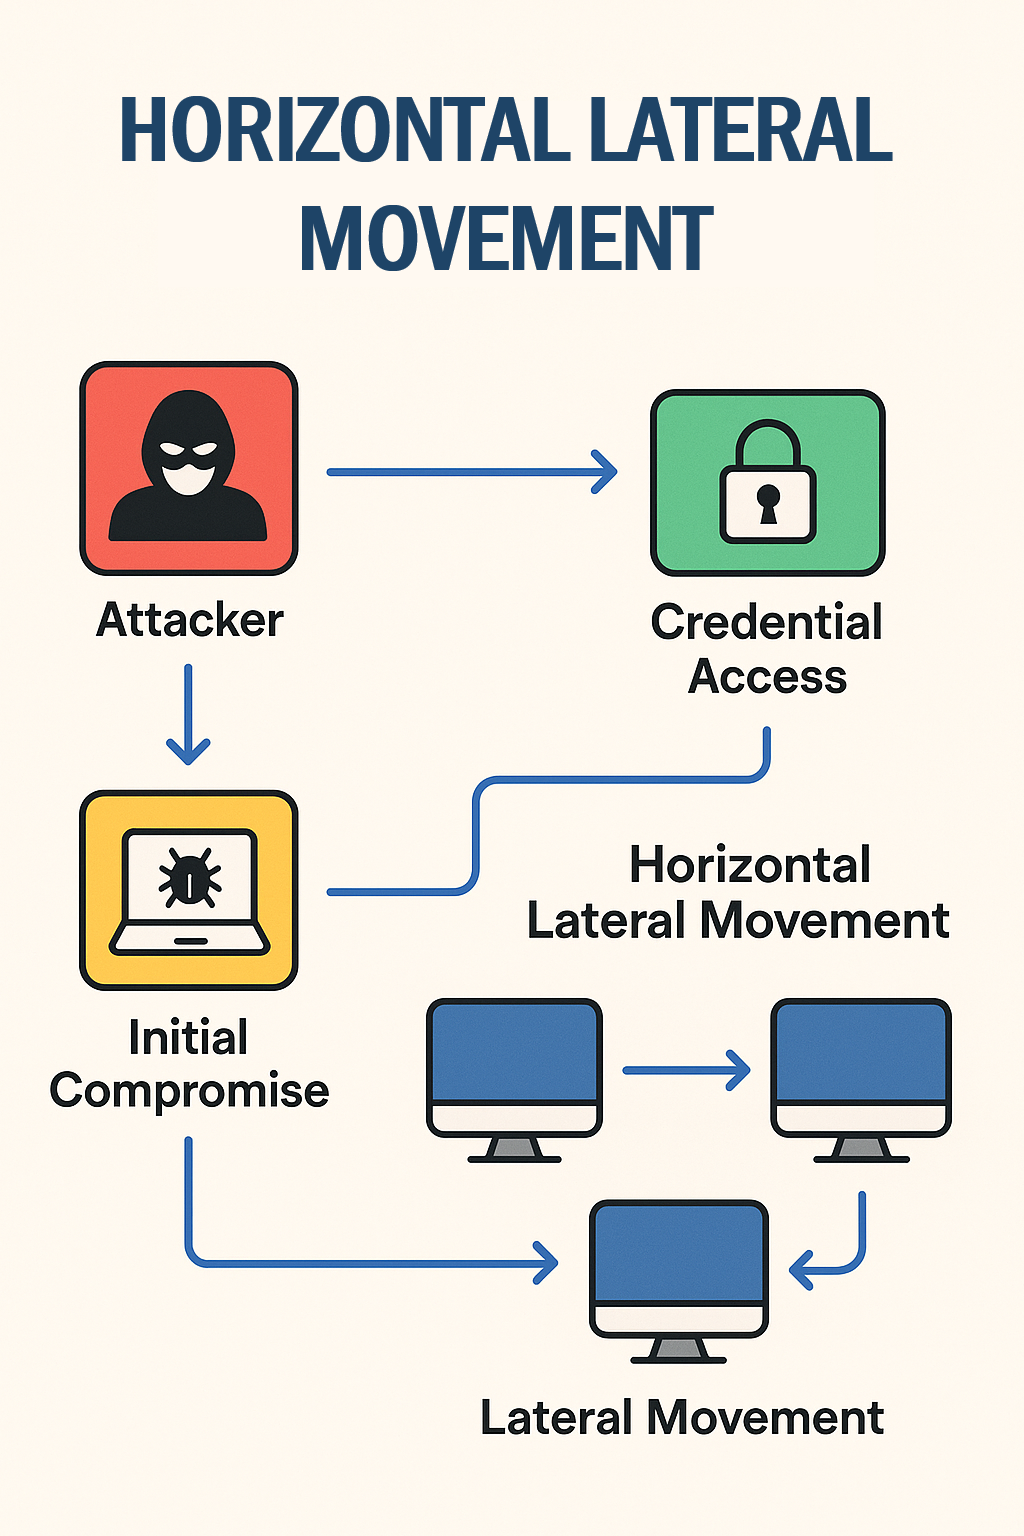
\includegraphics[width=0.5\linewidth]{horizontal-movement.png}
    \caption{Process diagram depicting horizontal lateral movement in a network}
    \label{fig:placeholder}
\end{figure}

\begin{figure}[H]
    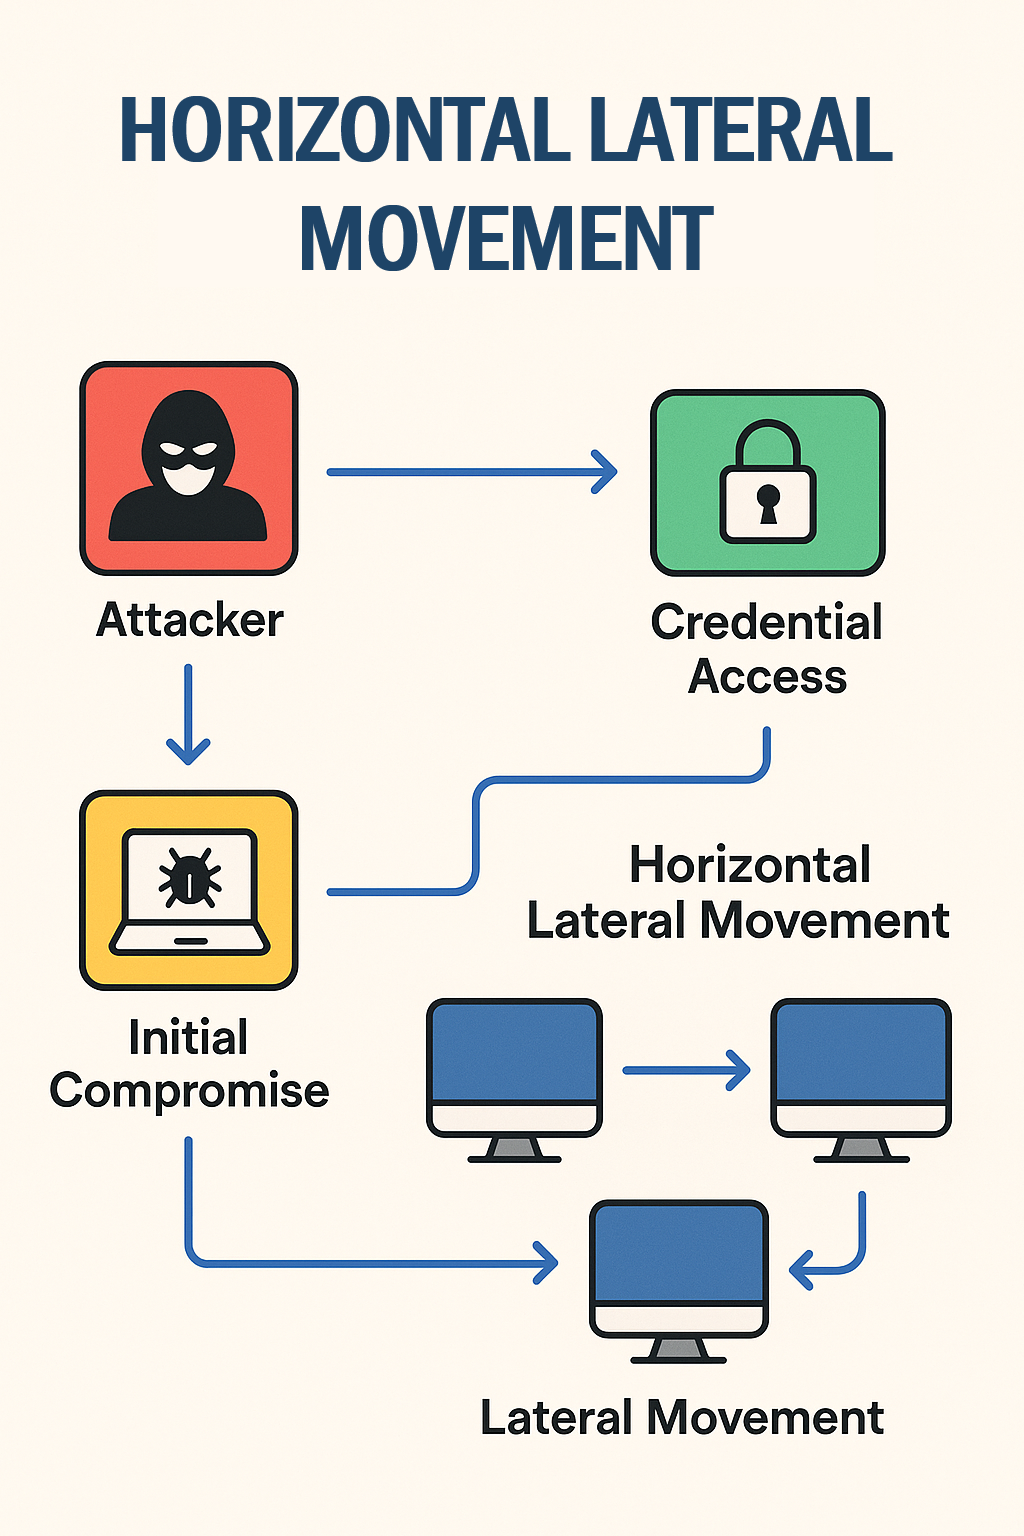
\includegraphics[width=0.5\linewidth]{horizontal-movement.png}
    \caption{Process diagram depicting horizontal lateral movement in a network}
    \label{fig:placeholder}
\end{figure}
    \begin{itemize}
        \item \textbf{Pass-the-Hash (PtH) Attack:} Attackers steal a password hash (a representation of a password), crack it offline to reveal its plaintext password, and then uses that password to impersonate the legitimate user and authenticate to other systems (as if the legitimate user) without needing the actual passwords that is commonly used in Windows environments.
        \item \textbf{SSH (Secure Shell) Hijacking:} Attackers may steal SSH keys or hijack existing SSH sessions to move between Linux, Unix, and Windows systems.
        \item \textbf{Trust Relationship Exploitation:} In networks with established trust between systems, for example, linked domains, attackers can exploit those relationships to move laterally without the need to re-authenticate.
    \end{itemize}


\section{2. Vertical Lateral Movement (Privilege Escalation)}
\begin{itemize}
    \item \textbf{Definition:} Involves escalating privileges or moving from a lower level of access to a higher level of access within a system or network. It aims to gain greater control and access to more deeply embedded sensitive information.
    \item \textbf{Goal:} To gain administrative access, root privileges, or access to sensitive data and systems with higher authority.


\begin{figure}[h]
    \centering
    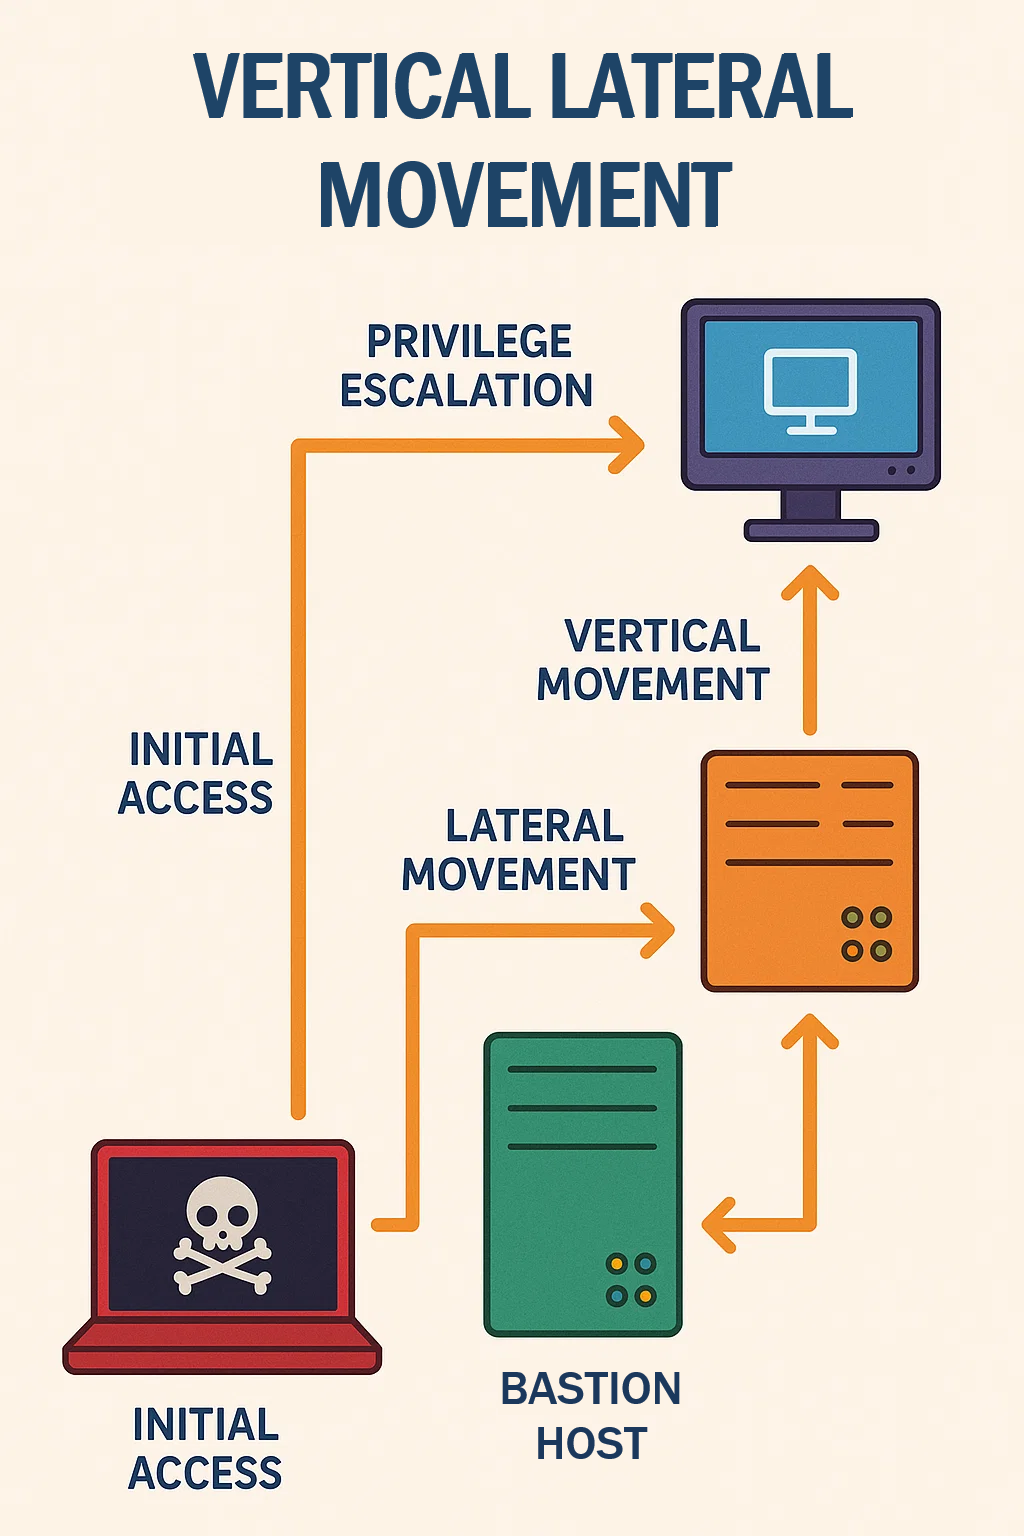
\includegraphics[width=0.5\linewidth]{vertical-movement.png}
    \caption{Process diagram depicting vertical lateral movement in a network}
    \label{fig:placeholder}
\end{figure}

    \item \textbf{Examples:}
    \begin{itemize}
        \item An attacker gains access to a standard user account and then exploits a software vulnerability to elevate their privileges to an administrator account.
        \item Exploiting a vulnerability in an outdated operating system or service to gain system-level control.
        \item An attacker compromises an application and uses its vulnerabilities or misconfigurations to gain administrative access to the underlying BIOS of the operating system.
        \item Using a legitimate user's credentials obtained successfully via a social engineering attack, such as phishing, an attacker can then leverage other vulnerabilities or misconfigurations to escalate privilege within the target system.

    \end{itemize}


\section{Understanding the Relationship Between the Two}
\begin{itemize}
    \item Lateral movement often involves both horizontal and vertical aspects.
    \item Attackers often begin with a horizontal move to expand their footprint and gather information about the target network, including potential targets and vulnerabilities.
    \item After expanding horizontally, they might then use vertical lateral movement to escalate privileges on specific target systems or accounts, granting them deeper access to sensitive data or critical infrastructure.

\end{itemize}

In essence, horizontal movement is about moving sideways within the network at a similar privilege level, while vertical movement is about moving upwards, gaining higher levels of access or control. Both are crucial stages in sophisticated cyberattacks and highlight the importance of layered security controlled approaches, detection strategies, situational and operational awareness, and incident response measures.









